% Author: Alfredo Sánchez Alberca (asalber@ceu.es)

\chapter{Probabilidad}

\section{Fundamentos teóricos}
\subsection{Introducción}
La estadística descriptiva permite describir el comportamiento y las relaciones entre las variables en la muestra, pero no permite sacar
conclusiones sobre el resto de la población.

Ha llegado el momento de dar el salto de la muestra a la población y pasar de la estadística descriptiva a la inferencia estadística, y el 
puente que lo permite es la \emph{teoría de la probabilidad}.

Hay que tener en cuenta que el conocimiento que se puede obtener de la población a partir de la muestra es limitado, pero resulta evidente
que la aproximación a la realidad de la población será mejor cuanto más representativa sea la muestra de ésta.
Y recordemos que para que la muestra sea representativa de la población deben utilizarse técnicas de muestreo aleatorio, es decir, en la que
los individuos se seleccionen al \emph{azar}.

La teoría de la probabilidad precisamente se encarga de controlar ese azar para saber hasta qué punto son fiables y extrapolables al
resto de la población las conclusiones obtenidas a partir de una muestra.

\subsection{Experimentos y sucesos aleatorios}
El estudio de una característica en una población se realiza a través de experimentos aleatorios.

\begin{definicion}[Experimento aleatorio] Un \emph{experimento aleatorio} es aquel en el que se conoce cuál es el conjunto de resultados
posibles antes de su realización pero se desconoce cuál será el resultado concreto del mismo.
\end{definicion}

Un ejemplo sencillo de experimentos aleatorios son los juegos de azar.
Por ejemplo, el lanzamiento de un dado es un experimento aleatorio ya que:
\begin{itemize}[label=--]
\item Se conoce el conjunto posibles de resultados $\{1,2,3,4,5,6\}$.
\item Antes de lanzar el dado, es imposible predecir con absoluta certeza el valor que saldrá. 
\end{itemize}

Otro ejemplo de experimento aleatorio sería la selección de un individuo de una población al azar y la determinación de su grupo sanguíneo.

En general, la obtención de cualquier muestra mediante procedimientos aleatorios será un experimento aleatorio.  

\begin{definicion}[Espacio muestral]
Al conjunto $E$ de todos los posibles resultados de un experimento aleatorio se le llama \emph{espacio muestral}.
\end{definicion}

Algunos ejemplos de espacios muestrales son:
\begin{itemize}
\item Lanzamiento de una moneda: $E=\{c,x\}$.
\item Lanzamiento de un dado: $E=\{1,2,3,4,5,6\}$.
\item Grupo sanguíneo de un individuo seleccionado al azar: $E=\{\mbox{A},\mbox{B},\mbox{AB},\mbox{0}\}$.
\item Estatura de un individuo seleccionado al azar: $\mathbb{R}^+$.
\end{itemize}

En los experimentos donde se miden más de una variable, la construcción del espacio muestral puede complicarse.
En tales casos, es recomendable utilizar un \emph{diagrama de árbol} de manera que cada nivel del árbol es una variable
observada y cada rama un posible valor.

Por ejemplo, si el experimento consiste en observar el sexo y el grupo sanguíneo de una persona, el espacio muestral podría construirse
mediante el siguiente árbol:

\begin{center}
\psset{treesep=0.2cm, levelsep=2cm}
\renewcommand{\psedge}[2]{\ncdiag[armA=0.7cm,angleA=180,angleB=0,armB=0cm]{#2}{#1}} 
\pstree[treemode=R, nodesep=1pt]{\Tp*}{
	\pstree[linestyle=none]{\TR[edge=none]{Sexo}}{\pstree{\TR{Grupo}}{\TR{$E$}}}
	\pstree{\TR{Mujer}}{
		\pstree[linestyle=none]{\TR{A}}{\TR{(Mujer,A)}}
		\pstree[linestyle=none]{\TR{B}}{\TR{(Mujer,B)}}
		\pstree[linestyle=none]{\TR{AB}}{\TR{(Mujer,AB)}}
		\pstree[linestyle=none]{\TR{0}}{\TR{(Mujer,0)}}
	}
	\pstree{\TR{Hombre}}{
		\pstree[linestyle=none]{\TR{A}}{\TR{(Hombre,A)}}
		\pstree[linestyle=none]{\TR{B}}{\TR{(Hombre,B)}}
		\pstree[linestyle=none]{\TR{AB}}{\TR{(Hombre,AB)}}
		\pstree[linestyle=none]{\TR{0}}{\TR{(Hombre,0)}}
	}
	\pstree[linestyle=none]{\Tp[edge=none]}{\Tp}
}
\end{center}

En RKWard los espacios muestrales se representan mediante conjuntos de datos con las variables que se midan en el experimento, indicando
en cada fila un resultado posible. 
Por ejemplo, el conjunto de datos correspondiente al espacio muestral del experimento anterior se muestra en la
figura~\ref{g:espacio_muestral}.

\begin{figure}[htp]
\begin{center}
  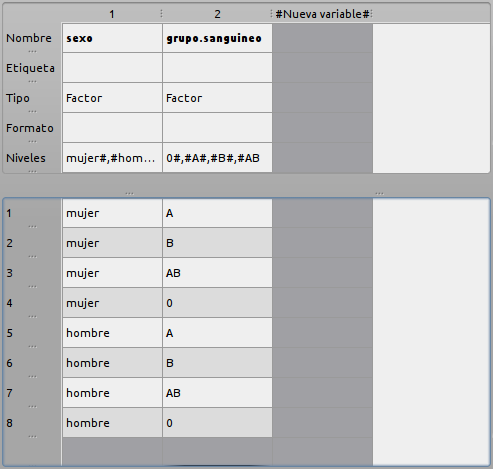
\includegraphics[scale=0.6]{probabilidad/img/espacio_muestral}
  \caption{Conjunto de datos correspondiente al espacio muestral del experimento consistente en sacar un individuo al azar de una población
  y medir su sexo y su grupo sanguíneo.}
  \label{g:espacio_muestral}
\end{center}
\end{figure}

\begin{definicion}[Suceso aleatorio]
Un \emph{suceso aleatorio} es cualquier subconjunto del espacio muestral $E$ de un experimento aleatorio. 
\end{definicion}

Existen distintos tipos de sucesos:
\begin{description}
\item[Suceso imposible:] Es el subconjunto vacío $\emptyset$. El suceso nunca ocurre.
\item[Sucesos elementales:] Son los subconjuntos formados por un solo elemento. 
\item[Sucesos compuestos:] Son los subconjuntos formados por dos o más elementos.
\item[Suceso seguro:] Es el propio espacio muestral. El suceso seguro siempre ocurre.
\end{description}

\begin{definicion}[Espacio de sucesos] Dado un espacio muestral $E$ de un
experimento aleatorio, el conjunto formado por todos los posibles sucesos de $E$ se llama \emph{espacio de sucesos de $E$} y se denota
$\mathcal{P}(E)$.
\end{definicion}

\begin{ejemplo}
Dado el espacio muestral $E=\{a,b,c\}$, se tiene 
\[
\mathcal{P}(E)=\left\{\emptyset, \{a\},\{b\},\{c\},\{a,b\},\{a,c\},\{b,c\},\{a,b,c\}\right\}
\]
\end{ejemplo}

Puesto que los sucesos son conjuntos, tiene sentido definir operaciones entre sucesos a partir de la teoría de conjuntos.

\begin{definicion}[Suceso unión]
Dados dos sucesos $A,B\in \mathcal{P}(E)$, se llama \emph{suceso unión} de $A$ y $B$, y se denota $A\cup B$, al suceso formado por los
elementos de $A$ junto a los elementos de $B$, es decir,
\[
A\cup B = \{x\,|\, x\in A\textrm{ o }x\in B\}.
\]
\begin{center}
\psset{unit=0.8}
\begin{pspicture}(-1,-1.5)(4,1.5)
\psset{fillstyle=solid}
\pscustom[fillcolor=white]{
\psframe(-1,-1.5)(4,1.5)}
\pscustom[fillcolor=yellow]{%
\psarc(1,0){1}{60}{-60}
\psarcn(2,0){1}{240}{120}}
\pscustom[fillcolor=yellow]{%
\psarc(2,0){1}{240}{120}
\psarcn(1,0){1}{60}{-60}}
\pscustom[fillcolor=yellow]{%
\psarc(1,0){1}{-60}{60}
\psarc(2,0){1}{120}{240}}
\rput(-0.7,1.2){$E$}
\rput(0.5,0){$A$}
\rput(1.5,-1.2){$A\cup B$}
\rput(2.5,0){$B$}
\end{pspicture}
\end{center}
\end{definicion}

El suceso unión $A\cup B$ ocurre siempre que ocurre $A$ \alert{o} $B$.

\begin{ejemplo}
Sea $E=\{1,2,3,4,5,6\}$, el conjunto de los números de un dado, y $A=\{2,4,6\}$ y $B=\{1,2,3,4\}$. 
Entonces $A\cup B=\{1,2,3,4,6\}$.
\end{ejemplo}

\begin{definicion}[Suceso intersección] 
Dados dos sucesos $A,B\in \mathcal{P}(E)$, se llama \emph{suceso intersección} de $A$ y $B$, y se denota $A\cap B$, al suceso formado por
los elementos comunes de $A$ y $B$, es decir, \[ A\cap B = \{x\,|\, x\in A\textrm{ y }x\in B\}.
\]
\begin{center}
\psset{unit=0.8}
\begin{pspicture}(-1,-1.5)(4,1.5)
\psset{fillstyle=solid}
\pscustom[fillcolor=white]{\psframe(-1,-1.5)(4,1.5)}
\pscustom[fillstyle=none]{%
\psarc(1,0){1}{60}{-60}
\psarcn(2,0){1}{240}{120}}
\pscustom[fillstyle=none]{%
\psarc(2,0){1}{240}{120}
\psarcn(1,0){1}{60}{-60}}
\pscustom[fillcolor=yellow]{%
\psarc(1,0){1}{-60}{60}
\psarc(2,0){1}{120}{240}}
\rput(-0.7,1.2){$E$}
\rput(0.5,0){$A$}
\rput(1.5,-1.2){$A\cap B$}
\rput(2.5,0){$B$}
\end{pspicture}
\end{center}
\end{definicion}

El suceso intersección $A\cap B$ ocurre siempre que ocurren $A$ \alert{y} $B$.

\begin{ejemplo}
Sea $E=\{1,2,3,4,5,6\}$, el conjunto de los números de un dado, y $A=\{2,4,6\}$ y $B=\{1,2,3,4\}$. 
Entonces $A\cap B=\{2,4\}$.
\end{ejemplo}

Diremos que dos sucesos son \structure{\textbf{incompatibles}} si su intersección es vacía.
Por ejemplo $A=\{2,4,6\}$ y $C=\{1,3\}$ son incompatibles.

\begin{definicion}[Suceso contrario]
Dado un conjunto $A\in \mathcal{P}(E)$, se llama \emph{suceso contrario o complementario} de $A$, y se denota $\bar A$, al suceso formado
por los elementos de $E$ que no pertenecen a $A$, es decir,
\[
\bar A = \{x\,|\, x\not\in A\}.
\]
\begin{center}
\psset{unit=0.8}
\begin{pspicture}(-1,-1.5)(4,1.5)
\psset{fillstyle=solid}
\pscustom[fillcolor=yellow]{
\psframe(-1,-1.5)(4,1.5)}
\pscustom[fillcolor=white]{%
\psarc(1,0){1}{0}{360}}
\rput(-0.7,1.2){$E$}
\rput(1,0){$A$}
\rput(3,0){$\bar A$}
\end{pspicture}
\end{center}
\end{definicion}

El suceso contrario $\bar A$ ocurre siempre que \alert{no} ocurre $A$.

\begin{ejemplo}
Sea $E=\{1,2,3,4,5,6\}$, el conjunto de los números de un dado, y $A=\{2,4,6\}$. 
Entonces $\overline A=\{1,3,5\}$.
\end{ejemplo}

\begin{definicion}[Suceso diferencia]
Dados dos sucesos $A,B\in \mathcal{P}(E)$, se llama \emph{suceso diferencia} de $A$ y $B$, y se denota $A-B$, al suceso formado por los elementos de $A$ que no pertenecen a $B$, es decir,
\[
A-B = \{x\,|\, x\in A\textrm{ y }x\not\in B\}.
\]
\begin{center}
\psset{unit=0.8}
\begin{pspicture}(-1,-1.5)(4,1.5)
\psset{fillstyle=solid}
\pscustom[fillcolor=white]{
\psframe(-1,-1.5)(4,1.5)}
\pscustom[fillcolor=yellow]{%
\psarc(1,0){1}{60}{-60}
\psarcn(2,0){1}{240}{120}}
\pscustom[fillstyle=none]{%
\psarc(2,0){1}{240}{120}
\psarcn(1,0){1}{60}{-60}}
\pscustom[fillstyle=none]{%
\psarc(1,0){1}{-60}{60}
\psarc(2,0){1}{120}{240}}
\rput(-0.7,1.2){$E$}
\rput(0.5,0){$A$}
\rput(1.5,-1.2){$A-B$}
\rput(2.5,0){$B$}
\end{pspicture}
\end{center}
\end{definicion}

El suceso diferencia $A-B$ ocurre siempre que ocurre $A$ pero no ocurre $B$, y también puede expresarse como $A\cap \bar B$.

\begin{ejemplo}
Sea $E=\{1,2,3,4,5,6\}$, el conjunto de los números de un dado, y $A=\{2,4,6\}$ y $B=\{1,2,3,4\}$. 
Entonces $A-B=\{6\}$ y $B-A=\{1,3\}$.
\end{ejemplo}

Dados los sucesos $A,B,C\in  \mathcal{P}(E)$, se cumplen las siguientes propiedades:
\begin{enumerate}
\item $A\cup A=A$, $A\cap A=A$ (idempotencia).
\item $A\cup B=B\cup A$, $A\cap B = B\cap A$ (conmutativa).
\item $(A\cup B)\cup C = A\cup (B\cup C)$, $(A\cap B)\cap C = A\cap (B\cap C)$ (asociativa).
\item $(A\cup B)\cap C = (A\cap C)\cup (B\cap C)$, $(A\cap B)\cup C = (A\cup C)\cap (B\cup C)$ (distributiva).
\item $A\cup \emptyset=A$, $A\cap E=A$ (elemento neutro).
\item $A\cup E=E$, $A\cap \emptyset=\emptyset$ (elemento absorbente).
\item $A\cup \bar A = E$, $A\cap \bar A= \emptyset$ (elemento simétrico complementario).
\item $\bar{\bar A} = A$ (doble contrario).
\item $\overline{A\cup B} = \bar A\cap \bar B$, $\overline{A\cap B} = \bar A\cup \bar B$ (leyes de Morgan).
\item $A\cap B\subseteq A\cup B$.
\end{enumerate}

\subsection{Definición de probabilidad}
En todo experimento aleatorio existe incertidumbre sobre el resultado de la realización del experimento. 
La probabilidad trata de cuantificar el grado de incertidumbre asociada a cada suceso de un experimento aleatorio. 
A lo largo de la historia se han utilizado distintas definiciones del concepto de probabilidad. 
A continuación se presentan las más comunes. 

\begin{definicion}[Probabilidad clásica de Laplace]
Para un experimento aleatorio donde todos los elementos del espacio muestral $E$ son equiprobables, se define la \emph{probabilidad} de un
suceso $A\subseteq E $ como el cociente entre el número de elementos de $A$ y el número de elementos de $E$:
\[ P(A) = \frac{|A|}{|E|} = \frac{\mbox{nº casos favorables a A}}{\mbox{nº casos posibles}}\]
\end{definicion}

\begin{ejemplo}
Si se considera el espacio muestral correspondiente al lanzamiento de un dado $E=\{1,2,3,4,5,6\}$, y el suceso correspondiente a sacar un
número par $A=\{2,4,6\}$, según la regla de Laplace, la probabilidad de sacar par al tirar un dado es
\[P(A)=\frac{|A|}{|E|}=\frac{3}{6}=0.5,\]
es decir, un 50\%. 
\end{ejemplo}

Esta definición es ampliamente utilizada, aunque tiene importantes restricciones:
\begin{itemize}[label=--]
\item No puede utilizarse con espacios muestrales infinitos, o de los que no se conoce el número de casos posibles.
\item Es necesario que todos los elementos del espacio muestral tengan la misma probabilidad de ocurrir (\emph{equiprobabilidad}).  
\end{itemize}

Estas restricciones suelen cumplirse en los experimentos relacionados con los juegos de azar (lanzamiento de dados, monedas, etc.) pero es
raro que ocurran en los experimentos de las ciencias de la salud.
Por ejemplo, los grupos sanguineos de una población humana no suelen ser equiprobables (normalmente el grupo A es mucho más probable que
el resto.)

En esto casos, y gracias al siguiente teorema, es mejor definir la probabilidad a partir de la frecuencia de cada suceso.

\begin{teorema}[Ley de los grandes números]
Cuando un experimento aleatorio se repite un gran número de veces, las frecuencias relativas de los sucesos del
experimento tienden a estabilizarse en torno a cierto número, que es precisamente su probabilidad.
\end{teorema}

Un ejemplo que demuestra el cumplimiento de esta ley puede realizarse tirando múltiples veces una moneda equilibrada y anotando la
frecuencia relativa de caras. 
A medida que se tire más veces la moneda se verá que la frecuencia relativa de caras se va estabilizando en torno a $0.5$ que es
la probabilidad de sacar cara. 

De acuerdo al teorema anterior, se puede dar la siguiente definición
\begin{definicion}[Probabilidad frecuentista]
Para un experimento aleatorio reproducible, se define la \emph{probabilidad} de un suceso $A\subseteq E $ como la frecuencia relativa del
suceso $A$ en infinitas repeticiones del experimento:
\[ P(A) = lim_{n\rightarrow \infty}\frac{n_{A}}{n}\]
\end{definicion}

\begin{ejemplo}
Si en una determinada población existe un 40\% de personas con grupo sanguíneo A, un 30\% de personas con grupo B, un 20\% con grupo 0 y un
10\% con grupo AB, de acuerdo a la definción frecuentista de probabilidad podemos decir que $P(A)=0.4$, $P(B)=0.3$, $P(0)=0.2$ y
$P(AB)=0.1$.
\end{ejemplo}

Aunque esta definición es muy útil en experimentos científicos reproducibles, también tiene serios inconvenientes, ya que
\begin{itemize}[label=--]
\item Sólo se calcula una aproximación de la probabilidad real.
\item La repetición del experimento debe ser en las mismas condiciones.  
\end{itemize}

No fue hasta el siglo XX cuando Kolmogórov dió una definición de probabilidad que unificaba las anteriores y que actualmente es la más
aceptada.

\begin{definicion}[Kolmogórov]
Se llama \emph{probabilidad} a toda aplicación que asocia a cada suceso $A$ del espacio de sucesos de un experimento aleatorio, un número
real $P(A)$, que cumple los siguientes axiomas:
\begin{enumerate}
\item La probabilidad de un suceso cualquiera es positiva o nula: \[P(A)\geq 0.\]
\item La probabilidad de la unión de dos sucesos incompatibles es igual a la suma de las probabilidades de cada uno de ellos:       
\[P(A\cup B) = P(A)+P(B).\]
\item La probabilidad del suceso seguro es igual a la unidad: 
\[P(E)=1.\]
\end{enumerate}
\end{definicion}

A partir de los axiomas de la definición de probabilidad se pueden deducir los siguientes resultados:
\begin{enumerate}
\item $P(\bar A) = 1-P(A)$.
\item $P(\emptyset)= 0$.
\item Si $A\subseteq B$ entonces $P(A)\leq P(B)$.
\item $P(A) \leq 1$.
\item Si $A$ y $B$ son sucesos compatibles, es decir, su intersección no es vacía, entonces 
\[P(A\cup B)= P(A) + P(B) - P(A\cap B).\]
\item Si el suceso $A$ está compuesto por los sucesos elementales $e_1,e_2,...,e_n$, entonces 
\[P(A)=\sum_{i=1}^n P(e_i).\]
\end{enumerate}

Este último resultado es especialmente interesante, pues pemite calcular la probabilidad de cualquier suceso de manera muy sencilla
simplemente sumando las probabilidades de los elementos que lo componen. 

\subsection{Probabilidad condicionada}
La incertidumbre sobre un suceso depende de la información que se tenga sobre el experimento aleatorio. 
En algunas ocasiones puede que haya que calcular la probabilidad de algún suceso $A$ sabiendo que ha ocurrido otro $B$. 
En tal caso se dice que el suceso $B$ es un \emph{condicionante}, y la probabilidad del suceso condicionado suele escribirse como 
\[P(A/B)\]

Los condicionantes, en el fondo, cambian el espacio muestral del experimento y por tanto las probabilidades de sus sucesos.

\begin{ejemplo}
Supongamos que hemos observado las siguientes frecuencias de fumadores en un grupo de 100 hombres y 100 mujeres:
\[
\begin{array}{|c|c|c|}
\cline{2-3}
 \multicolumn{1}{c|}{} & \mbox{Fuma} & \mbox{No Fuma} \\ \hline 
 \mbox{Mujeres} & 30 & 70 \\ \hline
 \mbox{Hombres} & 40 & 60 \\ \hline
 \mbox{Total} & 70 & 130 \\ \hline
\end{array}
\]
Entonces, utilizando la definición de frecuentista, la probabilidad de que una persona elegida al azar sea fumadora es
la frecuencia relativa de fumar que es $P(\mbox{Fumar})= 70/200=0.35$.

Sin embargo, si se añade información sobre el experimento y nos dicen que la persona elegida es mujer, entonces la muestra se restringiría
sólo a las mujeres y la frecuencia relativa de fumar en mujeres es $P(\mbox{Fumar}/\mbox{Mujer})=30/100=0.3$. 
\end{ejemplo}

El problema de los condicionamientos es que suelen cambiar el espacio muestral de partida. 
Afortunadamente, es posible calcular probabilidades condicionadas sin cambiar de espacio muestral gracias a la siguiente fórmula.

\begin{definicion}[Probabilidad condicionada]
Dados dos sucesos $A$ y $B$ de un mismo espacio de sucesos de un experimento aleatorio, la probabilidad de $A$ \emph{condicionada} por $B$
es 
\[ P(A/B) = \frac{P(A\cap B)}{P(B)},\]
siempre y cuando, $P(B)\neq 0$.
\end{definicion}

Esta definición permite calcular probabilidades sin tener que alterar el espacio muestral original del experimento.

\begin{ejemplo}
Siguiendo con el anterior, si se calcula la probabilidad de fumar en el caso de ser mujer con esta fórmula se obitne el mismo resultado:
\[P(\mbox{Fumar}/\mbox{Mujer})= \frac{P(\mbox{Fumar}\cap \mbox{Mujer})}{P(\mbox{Mujer})} = \frac{30/200}{100/200}=\frac{30}{100}=0.3.\]
\end{ejemplo}

De esta definición se deduce que la probabilidad de la intersección es
\[ P(A\cap B) = P(A)P(B/A) = P(B)P(A/B).\]

En ocasiones, saber que un determinado suceso ha ocurrido no cambia la incertidumbre sobre otro suceso del mismo experimento. 
Por ejemplo, si se tiran dos monedas, está claro que el resultado de la primera no cambia la incertidumbre sobre el resultado de la segunda.
En tal caso se dice que los sucesos son independientes.

\begin{definicion}[Sucesos independientes]
Dados dos sucesos $A$ y $B$ de un mismo espacio de sucesos de un experimento aleatorio, se dice que $A$ es \emph{independiente} de $B$, si
la probabilidad de $A$ no se ve alterada al condicionar por $B$, es decir,
\[ P(A/B) = P(A).\]
\end{definicion}

Si $A$ es independiente de $B$, también se cumple que $B$ es independiente de $A$, y en general simplemente se dice que $A$ y $B$ son
independientes.

También se cumple que si $A$ y $B$ son independientes, entonces 
\[ P(A\cap B) = P(A)P(B/A) = P(A)P(B). \]


\subsection{Espacios probabilísticos}
Si a cada uno de los elementos del espacio muestral de un experimento se le asocia su probabilidad, se obtiene un \emph{espacio
probabilístico}.

Resulta sencillo construir espacios probabilísticos a partir de los diagramas de árbol que se vieron para construir espacios muestrales. 
Para ello se deben etiquetar las ramas del árbol con probabilidades del siguiente modo: 
\begin{enumerate}
\item Para cada nodo del árbol, etiquetar su rama con la probabilidad de que la variable correspondiente tome el valor del nodo,
condicionada por la ocurrencia de todos los nodos que conducen hasta el actual.
\item La probabilidad de cada suceso elemental se calcula multiplicando las probabilidades que etiquetan las ramas que
conducen hasta él.
\end{enumerate}

\begin{ejemplo}[Espacio probabilístico con variables dependientes]
Sea una población en la que el 30\% de las personas fuman, y que la incidencia del cáncer de pulmón en fumadores es del 40\% mientras que 
en los no fumadores es del 10\%.

El espacio probabilístico de este experimento es:

\begin{center}
\psset{treesep=0.6cm, levelsep=3.5cm, tpos=0.6}
\renewcommand{\psedge}[2]{\ncdiag[armA=1.2cm,angleA=180,angleB=0,armB=0cm]{#2}{#1}} 
\pstree[treemode=R, nodesep=1pt]{\Tp*}{
	\pstree[linestyle=none]{\TR[edge=none]{Tabaco}}{
		\pstree{\TR{Enfermedad}}{
			\pstree{\TR{$E$}}{\TR{$P$}}
		}
	}
	\pstree{\TR{Fuma}\taput{\scriptsize $P(F)=0.3$}}{
		\pstree[linestyle=none]{\TR{Cáncer}\taput{\scriptsize $P(C/F)=0.4$}}{
			\pstree{\TR{(Fuma,Cáncer)}}{\TR{$0.3\cdot 0.4 = 0.12$}}
		}
		\pstree[linestyle=none]{\TR{$\overline{\mbox{Cáncer}}$}\taput{\scriptsize $P(\bar C/F)=0.6$}}{
			\pstree{\TR{(Fuma,$\overline{\mbox{Cáncer}}$)}}{\TR{$0.3\cdot 0.6 = 0.18$}}
		}
	}
	\pstree{\TR{$\overline{\mbox{Fuma}}$}\taput{\scriptsize $P(\bar F)=0.7$}}{
		\pstree[linestyle=none]{\TR{Cáncer}\taput{\scriptsize $P(C/\bar F)=0.1$}}{
			\pstree{\TR{($\overline{\mbox{Fuma}}$,Cáncer)}}{\TR{$0.7\cdot 0.1 = 0.07$}}
		}
		\pstree[linestyle=none]{\TR{$\overline{\mbox{Cáncer}}$}\taput{\scriptsize $P(\bar C/\bar F)=0.9$}}{
			\pstree{\TR{($\overline{\mbox{Fuma}}$,$\overline{\mbox{Cáncer}}$)}}{\TR{$0.7\cdot 0.9 = 0.63$}}
		}
	}
	\pstree[linestyle=none]{\Tp[edge=none]}{\Tp}
}
\end{center}

Obsérvese que el fumar o no depende del sexo, así que las ramas que salen del suceso mujer no tienen las mismas probabilidades que las que
salen del suceso hombre.
\end{ejemplo}

Cuando las variables observadas en el experimento son independientes, la construcción del espacio probabilístico se simplifica, ya que las
probabilidades condicionadas se convierten en probabilidades simples.

\begin{ejemplo}[Espacio probabilístico con variables independientes]
El espacio probabilístico del experimento aleatorio que consiste en el lanzamiento de dos monedas es:

\begin{center}
\psset{treesep=0.6cm, levelsep=2.5cm, tpos=0.7}
\renewcommand{\psedge}[2]{\ncdiag[armA=0.8cm,angleA=180,angleB=0,armB=0cm]{#2}{#1}} 
\pstree[treemode=R, nodesep=1pt]{\Tp*}{
	\pstree[linestyle=none]{\TR[edge=none]{1ª Moneda}}{\pstree{\TR{2ª Moneda}}{\pstree{\TR{$E$}}{\TR{$P$}}}}
	\pstree{\TR{C}\taput{\scriptsize $0.5$}}{
		\pstree[linestyle=none]{\TR{C}\taput{\scriptsize $0.5$}}{\pstree{\TR{(C,C)}}{\TR{$0.5\cdot 0.5 = 0.25$}}}
		\pstree[linestyle=none]{\TR{X}\taput{\scriptsize $0.5$}}{\pstree{\TR{(C,X)}}{\TR{$0.5\cdot 0.5 = 0.25$}}}
	}
	\pstree{\TR{X}\taput{\scriptsize $0.5$}}{
		\pstree[linestyle=none]{\TR{C}\taput{\scriptsize $0.5$}}{\pstree{\TR{(X,C)}}{\TR{$0.5\cdot 0.5 = 0.25$}}}
		\pstree[linestyle=none]{\TR{X}\taput{\scriptsize $0.5$}}{\pstree{\TR{(X,X)}}{\TR{$0.5\cdot 0.5 = 0.25$}}}
	}
	\pstree[linestyle=none]{\Tp[edge=none]}{\Tp}
}
\end{center}

Obsérvese ahora que el resultado de la segunda moneda no depende del resultado de la primera, de manera que las ramas que salen del suceso
cara en la primera moneda tienen las mismas probabilidades que las que salen del suceso cruz.
\end{ejemplo}  


\subsection{Teorema de la probabilidad total}
En algunos experimentos es posible descomponer el espacio muestral en partes que forman un sistema completo de sucesos. 

\begin{definicion}[Sistema completo de sucesos]
Una colección de sucesos $A_1,A_2,\ldots,A_n$ de un mismo espacio de sucesos es un \emph{sistema completo} si cumple las siguientes condiciones:
\begin{enumerate}
\item La unión de todos es el espacio muestral: $A_1\cup \cdots\cup A_n =E$.
\item Son incompatibles dos a dos: $A_i\cap A_j = \emptyset$ $\forall i\neq j$.
\end{enumerate}
\end{definicion}
\begin{center}
\psset{unit=0.8}
\begin{pspicture}(0,0)(5,3.5)
\psset{fillstyle=solid}
\pscustom[fillcolor=white]{\psframe(0,0)(5,3)}
\psline(1,0)(1,3)
\psline(2,0)(2,3)
\psline(4,0)(4,3)
\rput(0.5,1.5){$A_1$}
\rput(1.5,1.5){$A_2$}
\rput(3,1.5){$\cdots$}
\rput(4.5,1.5){$A_n$}
\rput[b](0.2,3.2){$E$}
\end{pspicture}
\end{center}

En realidad un sistema completo de sucesos es una partición del espacio muestral de acuerdo a algún atributo, como por ejemplo el sexo o el
grupo sanguíneo.

Conocer las probabilidades de un determinado suceso en cada una de las partes de un sistema completo puede ser útil para calcular su
probabilidad a partir del siguiente teorema.

\begin{teorema}[Probabilidad total]
Dado un sistema completo de sucesos $A_1,\ldots,A_n$ y un suceso $B$ de un mismo espacio de sucesos, se cumple
\[
P(B) = \sum_{i=1}^n P(A_i)P(B/A_i).
\]
\end{teorema}

\begin{center}
\psset{unit=1}
\begin{pspicture}(0,0)(5,3.5)
\psset{fillstyle=solid}
\pscustom[fillcolor=white]{\psframe(0,0)(5,3)}
\pscustom[fillcolor=coral]{\psellipse(2.5,1.5)(2,1)}
\psline(1,0)(1,3)
\psline(2,0)(2,3)
\psline(4,0)(4,3)
\rput(0.5,0.2){$A_1$}
\rput(1.5,0.2){$A_2$}
\rput(3,0.2){$\cdots$}
\rput(4.5,0.2){$A_n$}
\rput(3,1.5){$B$}
\rput[b](0.2,3.2){$E$}
\end{pspicture}
\end{center}

\begin{ejemplo}
Un determinado síntoma $B$ puede ser originado por una enfermedad $A$ pero también lo pueden presentar las personas sin
la enfermedad. 
Se sabe que en la población la tasa de personas con la enfermedad A es $0.2$. 
Además, de las personas que presentan la enfermedad, el $90\%$ presentan el síntoma, mientras que de las personas sin la enfermedad sólo lo
presentan el $40\%$.

Si se toma una persona al azar de la población, \emph{¿qué probabilidad hay de que tenga el síntoma?}

Para responder a la pregunta hay que fijarse en que el conjunto de sucesos $\{A,\bar A\}$ es un sistema completo, ya que $A\cup
\bar A = E$ y $A\cap \bar A = \emptyset$, de modo que se puede aplicar el teorema de la probabilidad total se tiene
\[ P(B) = P(A)P(B/A)+P(\bar A)P(B/\bar A) = 0.2\cdot 0.9 + 0.8\cdot 0.4 = 0.5.\] 
Es decir, la mitad de la población tendrá el síntoma.

En el fondo se trata de una media ponderada de probabilidades. 

La respuesta a la pregunta anterior es evidente a la luz del espacio probabilístico del experimento. 
\begin{center}
\psset{treesep=0.6cm, levelsep=2.5cm, tpos=0.6}
\renewcommand{\psedge}[2]{\ncdiag[armA=0.8cm,angleA=180,angleB=0,armB=0cm]{#2}{#1}} 
\pstree[treemode=R, nodesep=1pt]{\Tp*}{
	\pstree[linestyle=none]{\TR[edge=none]{Enfermedad}}{
		\pstree{\TR{Síntoma}}{
			\pstree{\TR{$E$}}{\TR{$P$}}
		}
	}
	\pstree{\TR{$A$}\taput{\scriptsize $0.2$}}{
		\pstree[linestyle=none]{\TR{$B$}\taput{\scriptsize $0.9$}}{
			\pstree{\TR{\alert{$(A,B)$}}}{\TR{\alert{$0.2\cdot 0.9 = 0.18$}}}
		}
		\pstree[linestyle=none]{\TR{$\bar B$}\taput{\scriptsize $0.1$}}{
			\pstree{\TR{$(A,\bar B)$}}{\TR{$0.2\cdot 0.1 = 0.02$}}
		}
	}
	\pstree{\TR{$\bar A$}\taput{\scriptsize $0.8$}}{
		\pstree[linestyle=none]{\TR{$B$}\taput{\scriptsize $0.4$}}{
			\pstree{\TR{\alert{$(\bar A,B)$}}}{\TR{\alert{$0.8\cdot 0.4 = 0.32$}}}
		}
		\pstree[linestyle=none]{\TR{$\bar B$}\taput{\scriptsize $0.6$}}{
			\pstree{\TR{$(\bar A,\bar B)$}}{\TR{$0.8\cdot 0.6 = 0.48$}}
		}
	}
	\pstree[linestyle=none]{\Tp[edge=none]}{\Tp}
}
\end{center}
\[
P(B) = P(A,B) + P(\bar A,B) = P(A)P(B/A)+P(\bar A)P(B/\bar A) = 0.2\cdot 0.9+ 0.8\cdot 0.4 = 0.18 + 0.32 = 0.5. 
\]
\end{ejemplo}


\subsection{Teorema de Bayes}
Los sucesos de un sistema completo de sucesos $A_1,\cdots,A_n$ también pueden verse como las distintas hipótesis ante un determinado hecho
$B$.

En estas condiciones puede ser útil calcular las probabilidades a posteriori $P(A_i/B)$ de cada una de las hipótesis, es decir, una vez
se haya cumplido el suceso $B$. 
Para ello se utiliza el teorema de Bayes. 

\begin{teorema}[Bayes]
Dado un sistema completo de sucesos $A_1,\ldots,A_n$ y un suceso $B$ de un mismo espacio de sucesos, se cumple
\[
P(A_i/B) = \frac{P(A_i\cap B)}{P(B)} = \frac{P(A_i)P(B/A_i)}{\sum_{i=1}^n P(A_i)P(B/A_i)}.
\]
\end{teorema}

\begin{ejemplo}[Diagnóstico de una enfermedad]
En el ejemplo anterior se ha visto cómo calcular la probabilidad de que una persona elegida al azar presente el síntoma, pero desde un 
punto de vista de diagnóstico clínico es mucho más interesante calcular la probabilidad de que una persona que presenta el síntoma tenga la
enfermedad, ya que esto permitiría diagnosticar la enfermedad o descartarla. 

En este caso, las hipótesis ante las que hay que decidir son $A$ y $\bar A$ y sus probabilidades ``a priori'' son $P(A)=0.2$ y
$P(\bar A)=0.8$.

Esto quiere decir que si no hubiese ninguna información sobre la persona, el diagnóstico sería que no tiene la enfermedad pues es mucho más
probable que que la tenga.

Sin embargo, si al reconocer a la persona se observa que presenta el síntoma, dicha información condiciona a las hipótesis, y para decidir
entre ellas es necesario calcular sus probabilidades ``a posteriori'', es decir 
\[ P(A/B) \mbox{ y } P(\bar A/B)\]

Para calcular estas probabilidades se puede utilizar el teorema de Bayes.
\begin{align*}
P(A/B) &= \frac{P(A)P(B/A)}{P(A)P(B/A)+P(\bar A)P(B/\bar A)} = \frac{0.2\cdot 0.9}{0.2\cdot 0.9 + 0.8\cdot 0.4} =
\frac{0.18}{0.5}=0.36,\\
P(\bar A/B) &= \frac{P(\bar A)P(B/\bar A)}{P(A)P(B/A)+P(\bar A)P(B/\bar A)} = \frac{0.8\cdot 0.4}{0.2\cdot 0.9 +
0.8\cdot 0.4} = \frac{0.32}{0.5}=0.64.
\end{align*}
Según esto, a pesar de que la probabilidad de estar enfermo ha aumentado, seguiríamos diagnosticando que no lo está, puesto que es más
probable.

En este caso se dice que el síntoma $B$ \emph{no es determinante} a la hora de diagnosticar la enfermedad, pues la información que aporta no
sirve para cambiar el diagnóstico en ningún caso.
\end{ejemplo}


\subsection{Tests diagnósticos}
En epidemiología es común el uso de tests para diagnosticar enfermedades.

Generalmente estos tests no son totalmente fiables, sino que hay cierta probabilidad de acierto o fallo en el diagnóstico, que suele
representarse en la siguiente tabla:
\begin{center}
\begin{tabular}{|m{3cm}<{\centering}|m{3.5cm}<{\centering}|m{3.5cm}<{\centering}|}
\cline{2-3}
\multicolumn{1}{c|}{} & Presencia de la\newline enfermedad ($E$) & Ausencia de la\newline enfermedad ($\overline E$)\\ \hline
Test positivo\newline ($+$) & \textcolor{green}{Diagnóstico acertado\newline  $P(+/E)$}\qquad
\structure{Sensibilidad}& \textcolor{red}{Diagnóstico erróneo\newline $P(+/\overline E)$}\\ \hline Test negativo\newline ($-$) &
\textcolor{red}{Diagnóstico erróneo\newline $P(-/E)$} & \textcolor{green}{Diagnóstico acertado\newline $P(-/\overline
E)$}\qquad \structure{Especificidad}\\ \hline
\end{tabular}
\end{center}

La valided de una prueba diagnóstica depende de estas dos probabilidades:
\begin{description}
\item[\textbf{Sensibilidad}] Es el porcentaje de positivos entre las personas enfermas: $P(+/E)$.
\item[\textbf{Especificidad}] Es el porcentaje de negativos entre las personas sanas: $P(-/\bar E)$.
\end{description}

Pero lo realmente interesante de un un test diagnóstico es su capacidad predictiva para diagnosticar, lo cual se mide mediante las
siguientes probabilidades a posteriori:
\begin{description}
\item[\textbf{Valor predictivo positivo}] Es el porcentaje de enfermos entre los positivos: $P(E/+)$.
\item[\textbf{Valor predictivo negativo}] Es el porcentaje de sanos entre los negativos: $P(\bar E/-)$.
\end{description}

Sin embargo, estos últmos valores dependen del porcentaje de enfermos en la población $P(E)$, lo que se conoce como, \emph{tasa
o prevalencia} de la enfermedad.

\begin{ejemplo}
Un test para diagnosticar la gripe tiene una sensibilidad del $95\%$ y una especificidad del $90\%$. 
Según esto, las probabilidades de
acierto y fallo del test son:
\begin{center}
\begin{tabular}{|c|c|c|}
\cline{2-3}
\multicolumn{1}{c|}{} & Gripe & No gripe\\ \hline
Test $+$ & $0.95$ & $0.10$\\ \hline
Test $-$ & $0.05$ & $0.90$\\ \hline
\end{tabular}
\end{center}

Si la prevalencia de la gripe en la población es del $10\%$ y al aplicar el test a un individuo da positivo, \emph{¿cuál es la probabilidad
de que tenga gripe?}

Aplicando el teorema de Bayes, se tiene que el valor predictivo positivo del test vale
\[
P(\mbox{Gripe}/+) = \frac{P(\mbox{Gripe})P(+/\mbox{Gripe})}{P(\mbox{Gripe})P(+/\mbox{Gripe})+P(\overline{\mbox{Gripe}})P(+/\overline{\mbox{Gripe}})}
= \frac{0.1\cdot 0.95}{0.1\cdot 0.95+0.9\cdot 0.1} = 0.5135.
\]
La probabilidad de no tener la gripe sería $P(\overline{\mbox{Gripe}})=1-0.51=0.49$, y como la probabilidad de tener la gripe es mayor que
la de no tenerla, se diagnosticaría que tiene gripe.
Sin embargo, el valor predictivo positivo de este test es muy bajo y nos equivoaríamos en el 49\% de los diagnósticos de enfermedad.

Y si el test da negativo, \emph{¿cuál es la probabilidad de que no tenga gripe?}

De nuevo, aplicando el teorema de Bayes, se tiene que el valor predictivo negativo del test vale
\[
P(\overline{\mbox{Gripe}}/-)=
\frac{P(\overline{\mbox{Gripe}})P(-/\overline{\mbox{Gripe}})}{P(\mbox{Gripe})P(-/\mbox{Gripe})+P(\overline{\mbox{Gripe}})P(-/\overline{\mbox{Gripe}})}
= \frac{0.9\cdot 0.9}{0.1\cdot 0.05+0.9\cdot 0.9} = 0.9939.
\]
De manera que el valor predictivo negativo de este test es mucho más alto que el valor predictivo positivo, y por tanto este test es mucho
más útil para descartar la enfermedad que para detectarla.
\end{ejemplo}


\clearpage
\newpage

\section{Ejercicios resueltos}
\begin{enumerate}[leftmargin=*] 
\item Construir los espacios muestrales correspondientes a los siguientes experimentos aleatorios:
\begin{enumerate}
\item Sacar una carta de una baraja española.
\begin{indicacion}{
\begin{enumerate}
\item Seleccionar el menú \menu{Teaching\flecha Probabilidad\flecha Juegos de azar\flecha Naipes\flecha Espacio probabilístico}.
\item En el cuadro de diálogo que aparece, desactivar la opción \opcion{Incluir probabilidades} y hacer clic en el botón \boton{Enviar}. 
\end{enumerate}
}
\end{indicacion}
\item Lanzar dos monedas.
\begin{indicacion}{
\begin{enumerate}
\item Seleccionar el menú \menu{Teaching\flecha Probabilidad\flecha Juegos de azar\flecha Monedas\flecha Espacio probabilístico}.
\item En el cuadro de diálogo que aparece, introducir 2 en el campo \campo{Número de monedas}, desactivar la opción \opcion{Incluir
probabilidades} y hacer clic en el botón \boton{Enviar}.
\end{enumerate}
}
\end{indicacion}

\item Lanzar dos dados.
\begin{indicacion}{
\begin{enumerate}
\item Seleccionar el menú \menu{Teaching\flecha Probabilidad\flecha Juegos de azar\flecha Dados\flecha Espacio probabilístico}.
\item En el cuadro de diálogo que aparece, introducir 2 en el campo \campo{Número de dados}, desactivar la opción \opcion{Incluir
probabilidades} y hacer clic en el botón \boton{Enviar}.
\end{enumerate}
}
\end{indicacion}

\item Lanzar dos dados y dos monedas. 
\begin{indicacion}{
\begin{enumerate}
\item Seleccionar el menú \menu{Teaching\flecha Probabilidad\flecha Combinar espacios probabilísticos independientes}.
\item En el cuadro de diálogo que aparece, seleccionar los conjuntos de datos correspondientes a los espacios muestrales del lanzamiento de
dos monedas y del lanzamiento de dos dados generados en los apartados anteriores, y hacer clic en el botón \boton{Enviar}.
\end{enumerate}
}
\end{indicacion}
\end{enumerate}  

\item Repetir el experimento de lanzar dos monedas 10 veces, 100 veces, 1000 veces y 1000000 de veces y calcular las frecuencias relativas
de cada resultado. 
¿Hacia dónde tienden las frecuencias? 
Construir el espacio probabilístico de este experimento y comprobar que se cumple la ley de los grandes números, es decir, que las
frecuencias anteriores se aproximan a las probabilidades de cada suceso elemental.
\begin{indicacion}{
Para la realización del experimento:
\begin{enumerate}
\item Seleccionar el menú \menu{Teaching\flecha Probabilidad\flecha Juegos de azar\flecha Monedas\flecha Lanzamiento de monedas}.
\item En el cuadro de diálogo que aparece, introducir 2 en el campo \campo{Número de monedas}, introducir 10 en el campo \campo{Número de
lanzamientos}, activar la casilla \opcion{Distribución de frecuencias} y hacer clic en el botón \boton{Enviar}.
\end{enumerate}
Repetir los mismos pasos pero introduciendo 100, 1000 y 1000000 respectivamente en el campo \opcion{Número de lanzamientos}.

Para construir el espacio probabilístico correspondiente:
\begin{enumerate}
\item Seleccionar el menú \menu{Teaching\flecha Probabilidad\flecha Juegos de azar\flecha Monedas\flecha Espacio probabilístico}.
\item En el cuadro de diálogo que aparece, introducir 2 en el campo \campo{Número de monedas} y hacer clic en el botón \boton{Enviar}.
\end{enumerate}
}
\end{indicacion}

\item En una estantería hay tres cajas de un medicamento A, dos de un medicamento B y una de un medicamento C. 
Construir los espacios probabilísticos asociados a los siguientes experimentos aleatorios:
\begin{enumerate}
\item Elegir tres medicamentos al azar sin reemplazamiento. 
\begin{indicacion}{
\begin{enumerate}
\item Seleccionar el menú \menu{Teaching\flecha Probabilidad\flecha Juegos de azar\flecha Urna\flecha Espacio probabilístico}.
\item En el cuadro de diálogo que aparece, seleccionar la opción \opcion{Lista de objetos}, introducir los objetos A,A,A,B,B,C en
el campo \campo{Lista de objetos}, introducir 3 en el campo \campo{Número de extracciones}, y hacer clic en el botón \boton{Enviar}.
\end{enumerate}
}
\end{indicacion}

\item Elegir tres medicamentos al azar con reemplazamiento.
\begin{indicacion}{
Repetir los mismos pasos del apartado anterior pero además activando la casilla \opcion{Con reemplazamiento}.
}
\end{indicacion}
\end{enumerate}

\item En una población se ha hecho un estudio epidemiológico sobre tres enfermedades asociadas habitualmente a la infancia, como son la
varicela, el sarampión y la rubeola.
Las frecuencias observadas aparecen en la siguiente tabla:
\begin{center}
\begin{tabular}{cccr}
\hline
Varicela & Sarampión & Rubeola & Frecuencia\\
No & No & No & 2654\\
No & No & Si & 1436\\
No & Si & No & 1682\\
No & Si & Si & 668\\
Si & No & No & 1747\\
Si & No & Si & 476\\
Si & Si & No & 876\\
Si & Si & Si & 265\\
\hline
\end{tabular}
\end{center}

Se pide:
\begin{enumerate}
\item Crear el conjunto de datos \variable{enfermedades.infantiles} con las variables \variable{varicela}, \variable{sarampion},
\variable{rubeola} y \variable{frecuencia} e introducir datos de la población.

\item Crear el espacio probabilístico asociado a la población.
\begin{indicacion}{
\begin{enumerate}
\item Seleccionar el menú \menu{Teaching\flecha Probabilidad\flecha Construir espacio probabilístico}.
\item En el cuadro de diálogo que aparece seleccionar el conjunto de datos \variable{enfermedades.infantiles}, activar la casilla
\opcion{Definir frecuencias}, seleccionar la variable \variable{frecuencia} en el campo \campo{Frecuencia}, darle el nombre
\variable{enfermedades.infantiles.ep} al espacio probabilístico y hacer clic en el botón \boton{Enviar}.
\end{enumerate}
}
\end{indicacion}  

\item Calcular la probabilidad de que una persona de esta población haya tenido varicela. 
\begin{indicacion}{
\begin{enumerate}
\item Seleccionar el menú \menu{Teaching\flecha Probabilidad\flecha Calcular probabilidad}.
\item En el cuadro de diálogo que aparece seleccionar el espacio probabilístico \variable{enfermedades.infantiles.ep}, introducir
\comando{varicela == "Si"} en el campo \campo{Suceso} y hacer clic en el botón \boton{Enviar}.
\end{enumerate}
}
\end{indicacion} 

\item Calcular la probabilidad de que una persona de esta población haya tenido varicela o sarampión. 
\begin{indicacion}{
\begin{enumerate}
\item Seleccionar el menú \menu{Teaching\flecha Probabilidad\flecha Calcular probabilidad}.
\item En el cuadro de diálogo que aparece seleccionar el espacio probabilístico \variable{enfermedades.infantiles.ep}, introducir
\comando{varicela == "Si" | sarampion=="Si"} en el campo \campo{Suceso} y hacer clic en el botón \boton{Enviar}.
\end{enumerate}
}
\end{indicacion} 

\item Calcular la probabilidad de que una persona de esta población haya tenido sarampión y rubeola. 
\begin{indicacion}{
\begin{enumerate}
\item Seleccionar el menú \menu{Teaching\flecha Probabilidad\flecha Calcular probabilidad}.
\item En el cuadro de diálogo que aparece seleccionar el espacio probabilístico \variable{enfermedades.infantiles.ep}, introducir
\comando{sarampion == "Si" & rubeola=="Si"} en el campo \campo{Suceso} y hacer clic en el botón \boton{Enviar}.
\end{enumerate}
}
\end{indicacion} 

\item Calcular la probabilidad de que una persona de esta población haya tenido varicela si no ha tenido sarampion.
¿Son independientes el haber tenido varicela y el haber tenido sarampión? 
\begin{indicacion}{
\begin{enumerate}
\item Seleccionar el menú \menu{Teaching\flecha Probabilidad\flecha Calcular probabilidad}.
\item En el cuadro de diálogo que aparece seleccionar el espacio probabilístico \variable{enfermedades.infantiles.ep}, introducir
\comando{varicela == "Si"} en el campo \campo{Suceso}, activar la casilla \opcion{Probabilidad condicionada}, introducir \comando{sarampion
== "No"} en el campo \campo{Condición} y hacer clic en el botón \boton{Enviar}.
\end{enumerate}
}
\end{indicacion} 

\item Calcular la probabilidad de que una persona de esta población no haya tenido rubeola ni sarampión si ha tenido varicela. 
\begin{indicacion}{
\begin{enumerate}
\item Seleccionar el menú \menu{Teaching\flecha Probabilidad\flecha Calcular probabilidad}.
\item En el cuadro de diálogo que aparece seleccionar el espacio probabilístico \variable{enfermedades.infantiles.ep}, introducir
\comando{rubeola == "No" & sarampion=="No"} en el campo \campo{Suceso}, activar la casilla \opcion{Probabilidad condicionada}, introducir
\comando{varicela == "Si"} en el campo \campo{Condición} y hacer clic en el botón \boton{Enviar}.
\end{enumerate}
}
\end{indicacion} 
\end{enumerate}

\item Se ha probado un test diagnóstico para detectar el embarazo en un grupo de mujeres en edad de procrear, obteniendo los siguientes
resultados
\begin{center}
\begin{tabular}{ccr}
\hline
Embarazo & Test & Frecuencia\\ 
No & $-$ & 3876\\
No & $+$ & 47\\
Si & $-$ & 12\\
Si & $+$ & 131\\
\hline
\end{tabular}
\end{center}
Se pide:
\begin{enumerate}
\item Crear el conjunto de datos \variable{test.embarazo} con las variables \variable{embarazo}, \variable{test}, y \variable{frecuencia} e
introducir datos de la muestra.
\item Crear el espacio probabilístico asociado a la población.
\begin{indicacion}{
\begin{enumerate}
\item Seleccionar el menú \menu{Teaching\flecha Probabilidad\flecha Construir espacio probabilístico}.
\item En el cuadro de diálogo que aparece seleccionar el conjunto de datos \variable{test.embarazo}, activar la casilla
\opcion{Definir frecuencias}, seleccionar la variable \variable{frecuencia} en el campo \campo{Frecuencia}, darle el nombre
\variable{test.embarazo.ep} al espacio probabilístico y hacer clic en el botón \boton{Enviar}.
\end{enumerate}
}
\end{indicacion}  

\item Calcular la prevalencia del embarazo.
\begin{indicacion}{
\begin{enumerate}
\item Seleccionar el menú \menu{Teaching\flecha Probabilidad\flecha Calcular probabilidad}.
\item En el cuadro de diálogo que aparece seleccionar el espacio probabilístico \variable{test.embarazo.ep}, introducir
\comando{embarazo == "Si"} en el campo \campo{Suceso} y hacer clic en el botón \boton{Enviar}.
\end{enumerate}
}
\end{indicacion} 

\item Calcular la probabilidad de que el test de positivo.
\begin{indicacion}{
\begin{enumerate}
\item Seleccionar el menú \menu{Teaching\flecha Probabilidad\flecha Calcular probabilidad}.
\item En el cuadro de diálogo que aparece seleccionar el espacio probabilístico \variable{test.embarazo.ep}, introducir
\comando{test == "+"} en el campo \campo{Suceso} y hacer clic en el botón \boton{Enviar}.
\end{enumerate}
}
\end{indicacion} 

\item Calcular la sensibilidad del test.
\begin{indicacion}{
\begin{enumerate}
\item Seleccionar el menú \menu{Teaching\flecha Probabilidad\flecha Calcular probabilidad}.
\item En el cuadro de diálogo que aparece seleccionar el espacio probabilístico \variable{test.embarazo.ep}, introducir
\comando{test=="+"} en el campo \campo{Suceso}, activar la casilla \opcion{Probabilidad condicionada}, introducir
\comando{embarazo == "Si"} en el campo \campo{Condición} y hacer clic en el botón \boton{Enviar}.
\end{enumerate}
}
\end{indicacion} 

\item Calcular la especificidad del test.
\begin{indicacion}{
\begin{enumerate}
\item Seleccionar el menú \menu{Teaching\flecha Probabilidad\flecha Calcular probabilidad}.
\item En el cuadro de diálogo que aparece seleccionar el espacio probabilístico \variable{test.embarazo.ep}, introducir
\comando{test=="-"} en el campo \campo{Suceso}, activar la casilla \opcion{Probabilidad condicionada}, introducir
\comando{embarazo == "No"} en el campo \campo{Condición} y hacer clic en el botón \boton{Enviar}.
\end{enumerate}
}
\end{indicacion} 

\item Calcular el valor predictivo positivo del test. 
¿Es útil el test para detectar la enfermedad? 
\begin{indicacion}{
\begin{enumerate}
\item Seleccionar el menú \menu{Teaching\flecha Probabilidad\flecha Calcular probabilidad}.
\item En el cuadro de diálogo que aparece seleccionar el espacio probabilístico \variable{test.embarazo.ep}, introducir
\comando{embarazo=="Si"} en el campo \campo{Suceso}, activar la casilla \opcion{Probabilidad condicionada}, introducir
\comando{test=="+"} en el campo \campo{Condición} y hacer clic en el botón \boton{Enviar}.
\end{enumerate}
}
\end{indicacion} 

\item Calcular el valor predictivo negativo del test.
¿Es útil el test para descartar la enfermedad?
\begin{indicacion}{
\begin{enumerate}
\item Seleccionar el menú \menu{Teaching\flecha Probabilidad\flecha Calcular probabilidad}.
\item En el cuadro de diálogo que aparece seleccionar el espacio probabilístico \variable{test.embarazo.ep}, introducir
\comando{embarazo=="No"} en el campo \campo{Suceso}, activar la casilla \opcion{Probabilidad condicionada}, introducir
\comando{test=="-"} en el campo \campo{Condición} y hacer clic en el botón \boton{Enviar}.
\end{enumerate}
}
\end{indicacion} 
\end{enumerate} 

\end{enumerate}


\section{Ejercicios propuestos}
\begin{enumerate}[leftmargin=*]
\item Construir el espacio muestral correspondiente a tirar una moneda, un dado y sacar una carta de una baraja española. 

\item Para comprobar la eficacia de una vacuna contra la gripe se tomó una muestra de 1000 y se observó si fueron vacunadas y si finalmente
tuvieron gripe o no. 
Los resultados obtenidos fueron los siguientes
\begin{center}
\begin{tabular}{ccr}
\hline
Vacuna & Gripe & Frecuencia\\
No & No & 418\\
No & Si & 312\\
Si & No & 233\\
Si & Si & 37\\
\hline
\end{tabular}
\end{center}
Se pide:
\begin{enumerate}
\item Construir el espacio probabilístico asociado al experimento.
\item Calcular la probabilidad de haberse vacunado contra la gripe.  
\item Calcular la prevalencia de la gripe.
\item Calcular la probabilidad de desarrollar la gripe tras haberse vacunado.
¿Es efectiva la vacuna?
\end{enumerate}

\item Para probar la eficacia de un test diagnóstico para dectectar el ébola en un país centroafricano, se tomó una muestra de personas
a las que se le ha aplicado el test. 
El test dió positivo en 147 personas con ébola, pero también dió positivo en 28 personas sin ébola. 
Por otro lado el test dió negativo en 97465 personas sin ébola, pero también dió negativo en 65 personas con ébola.
Se pide:
\begin{enumerate}
\item Construir el espacio probabilístico asociado al test diagnóstico.
\item Calcula la prevalencia del ébola en ese país.
\item Calcular la probabilidad de que el test de negativo. 
\item Calcular la sensibilidad y la especificidad del test.  
\item ¿Para qué es más efectivo el test, para dectectar o para descartar el ébola?
\end{enumerate} 
\end{enumerate}







